\documentclass{article}
\usepackage[T1]{fontenc}
\usepackage{lmodern}
\usepackage{graphicx}
\usepackage{amsmath,amssymb}
\usepackage[a4paper,margin=2cm]{geometry}
\usepackage[absolute,overlay]{textpos}
\setlength{\TPHorizModule}{1mm}
\setlength{\TPVertModule}{1mm}
\usepackage[indonesian]{babel}
\usepackage{hyperref}
\setlength{\emergencystretch}{2em}
% unit: Halaman 23

\begin{document}

% === Halaman 23 (llm) ===

\vspace{132.16mm}

Beberapa adegan film \textit{Beautiful Mind} yang memperlihatkan steganografi

\vspace{130.68mm}

% deskripsi: Screenshot adegan film A Beautiful Mind yang menunjukkan layar dengan banyak teks dan kode, dengan subtitle 'Ever just know something, Dr. Nash?'
% bbox normalisasi: [0.1180, 0.0530, 0.5200, 0.4980]
\begin{textblock*}{84.42mm}(24.78mm,15.74mm)
\noindent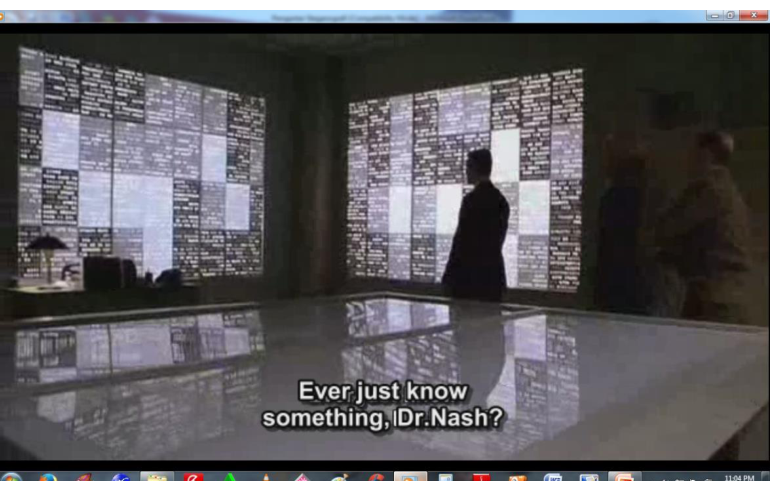
\includegraphics[width=84.42mm,height=132.16mm]{../../images/llm/page_023_img_01.png}%
\end{textblock*}

% deskripsi: Screenshot adegan film A Beautiful Mind yang menunjukkan teks 'ARTIFICIAL LIFE' dalam sebuah dokumen.
% bbox normalisasi: [0.4610, 0.5280, 0.8830, 0.9680]
\begin{textblock*}{88.62mm}(96.81mm,156.82mm)
\noindent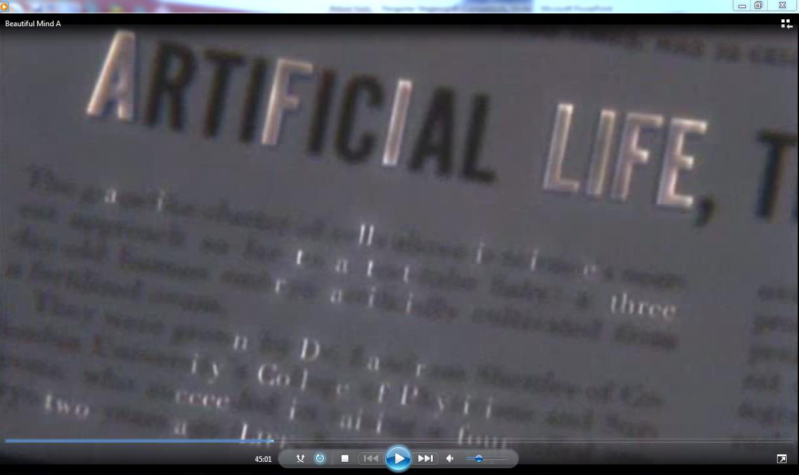
\includegraphics[width=88.62mm,height=130.68mm]{../../images/llm/page_023_img_02.png}%
\end{textblock*}

\end{document}
